\section{Idea \& Implementation}

\subsection{Idea}

\noindent The main idea can be split into the following steps (which also are
the states of the main controller, \hl{SwarmRobotics.lua}).

\begin{enumerate}
    \item Initialization
    \item Robots split into rooms by going to the nearest room. It does not
    ensure that a robot of each type will be in each room (see Analysis \&
    Problems section).
    \item Go towards target: light source for light robots, and door step for
    ground robots. Compute the 3 values to evaluate the room.
    \item Robots go towards farther robots in order to exit the current room.
    They group themselves inside the central room and share partial scores to
    obtain total score for their assignated room. Once total scores are computed,
    they can be shared to decide which is the best one.
    \item Go towards the best detected room.
\end{enumerate}

\subsection{Implementation details}

\subsubsection{MoveIntoRoom}

The \hl{MoveIntoRoom.lua} state machine has for purpose to let robots go towards
a room and detect when the robot is inside said room. First, the robot is
attracted by the door associated with the room. When the robot is close enough
to the door (1st threshold), then it is attracted by elements inside the room
(objects and light source). Once a 2nd threshold has been reached, the robot is
considered inside the room.

\subsubsection{TargetRoomFormation}

The \hl{TargetRoomFormation.lua} has for purpose to let robots go towards their
target once inside a room. Light robots go towards the light source and Ground
robots go towards the door step. Moreover, a vector reprensenting robots
interaction is computed using the Lennard-Jones force. This is done in order
to avoid robots blocking each other (repulsion), while keeping them close to
avoid unecessary wandering.

\subsubsection{Message channels}

The following bytes have been reserved for the range\_and\_bearing system to
exchange messages (see \hl{MsgBytes.lua}).

\begin{enumerate}
    \item ping, notify position of current robot to other robots, used for
    pattern formation
    \item red, red component of a room's color
    \item green, green component of a room's color
    \item blue, blue component of a room's color
    \item L robot partial score (light intensity + objects evaluation)
    \item G robot partial score (ground evaluation)
    \item associated room's total score
\end{enumerate}

\subsection{Main steps}

\begin{figure}[h!]
        \centering
        \begin{subfigure}[b]{0.5\textwidth}
            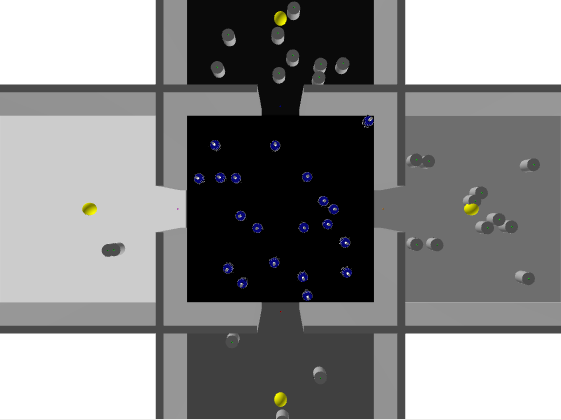
\includegraphics[width=\textwidth]{images/1_start.png}
            \caption{Start}
        \end{subfigure}%
        ~
        \begin{subfigure}[b]{0.5\textwidth}
            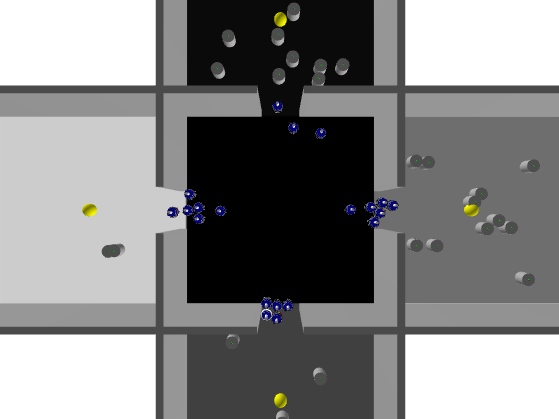
\includegraphics[width=\textwidth]{images/2_split.png}
            \caption{Split}
        \end{subfigure}
        \hfill
        \begin{subfigure}[b]{0.5\textwidth}
            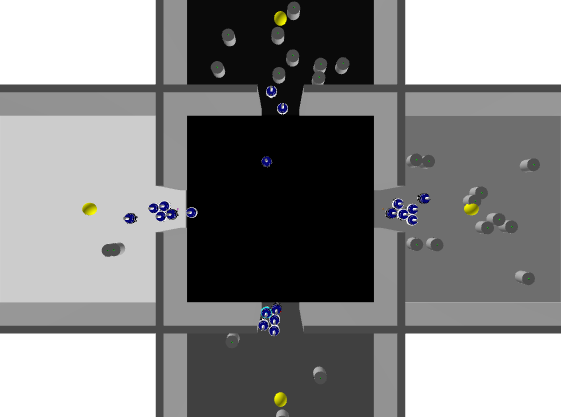
\includegraphics[width=\textwidth]{images/3_evaluate.png}
            \caption{Room evaluation}
        \end{subfigure}%
        ~
        \begin{subfigure}[b]{0.5\textwidth}
            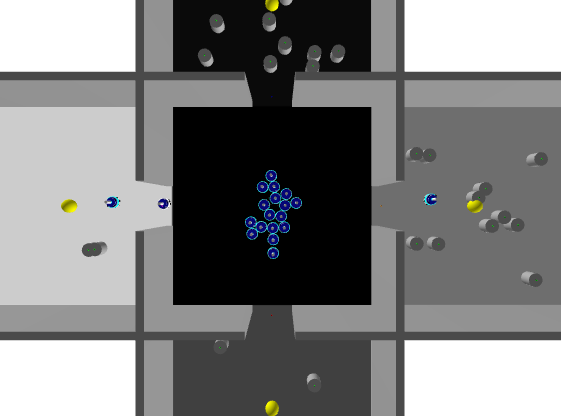
\includegraphics[width=\textwidth]{images/4_sync.png}
            \caption{Gathering \& scores sync}
        \end{subfigure}
        \hfill
        \begin{subfigure}[b]{0.5\textwidth}
            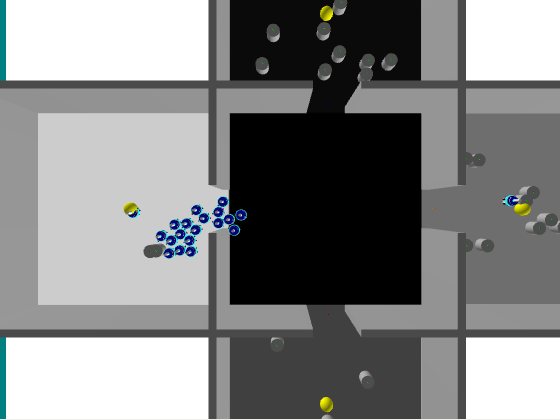
\includegraphics[width=\textwidth]{images/5_best.png}
            \caption{Go to best room}
        \end{subfigure}
        \caption{Main steps}\label{fig:steps}
\end{figure}

% TODO screenshots steps
\newpage
